% =====================================================================
%  Shared sections (model, stability, control, swing-up) used by build_full_report.py and build_phase_reports.py
%  (layout follows the senior reference report: title page, contents,
%   numbered sections, code listings, tabulation, conclusion, contributions)
% =====================================================================
\documentclass[12pt,a4paper]{article}
\usepackage[a4paper,margin=1in]{geometry}
\usepackage[T1]{fontenc}
\usepackage{lmodern}
\usepackage{amsmath,amssymb,bm}
\usepackage{graphicx,float,booktabs,array,multirow}
\usepackage{xcolor}
\usepackage{algorithm}
\usepackage{algpseudocode}
\usepackage{fancyhdr}
\usepackage{enumitem}
\usepackage{caption}
\usepackage[hidelinks]{hyperref}

\pagestyle{fancy}
\fancyhf{}
\renewcommand{\headrulewidth}{0.6pt}
\fancyfoot[C]{\thepage}
\setlength{\headheight}{14.5pt}
\setlength{\parskip}{4pt}
\setlength{\parindent}{0pt}
\newcommand{\Nm}{\,\mathrm{N\,m}}
\captionsetup{font=small}

\begin{document}

\begin{titlepage}
\centering
\vspace*{2cm}

\includegraphics[width=4.2cm]{figures/logo-000.jpg}\\[3cm]
{\Huge Systems Thinking Project}\\[0.5cm]
{\Large Acrobot}\\[0.25cm]
{\large Phase 2: Stability Analysis}\\[2.2cm]
\begin{tabular}{cc}
\textbf{Author:} Bhargav & \textbf{Author:} Sreekar\\
ID: 2025102061 & ID: 2025102074\\[0.8cm]
\textbf{Author:} Kaushik & \textbf{Author:} Divijat\\
ID: 2025102071 & ID: 2025102040
\end{tabular}
\vfill
{\large November 11, 2026}
\end{titlepage}

\tableofcontents
\newpage

\section{Introduction}
% =====================================================================
\subsection{What is an Acrobot?}
An acrobot is a two-link pendulum that hangs from a fixed pivot. The first link (the ``shoulder'' link) is free to rotate about the pivot; the second link is joined to the end of the first at the ``elbow''. The only motor sits at the elbow, so the shoulder is \emph{passive}. It is the robot version of a gymnast on a high bar who can only swing the legs at the hips. Because there are two degrees of freedom but only one actuator, the acrobot is a standard example of an \emph{underactuated} system [1], [2].

\subsection{Model}
The configuration is described by two generalised coordinates: $q_1$, the angle of link~1 from the downward vertical, and $q_2$, the angle of link~2 relative to link~1. The full state contains the angles and their rates:
\[
\mathbf q=\begin{bmatrix}q_1\\q_2\end{bmatrix},\qquad
\mathbf x=\begin{bmatrix}q_1\\q_2\\\dot q_1\\\dot q_2\end{bmatrix}.
\]
\begin{figure}[H]
\centering
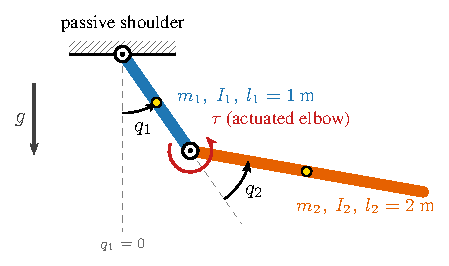
\includegraphics[width=0.42\textwidth]{figures/acrobot_diagram.pdf}
\caption{The acrobot: passive shoulder at the pivot, motor torque $\tau$ at the elbow; dots mark the centres of mass.}
\label{fig:acrobot}
\end{figure}

\subsection{Equations of Motion}
The dynamics (given in the Phase~1 helper and verified in Phase~1) are
\begin{equation}
M(q)\,\ddot q+C(q,\dot q)\,\dot q=\tau_g(q)+B\,\tau,\qquad B=\begin{bmatrix}0\\1\end{bmatrix},\qquad |\tau|\le 20\Nm .\label{eq:eom}
\end{equation}

\textbf{$\tau$ (Input Torque):} the torque of the elbow motor, the only quantity we command. $B=[0,\,1]^T$ says it acts on the elbow equation only.

\textbf{$M(q)$ (Inertia Matrix):} the resistance to angular acceleration. It depends on the elbow angle because the mass distribution changes as the arm folds:
\begin{equation}
M(q)=\begin{bmatrix}2.663+2\cos q_2 & 1.33+\cos q_2\\ 1.33+\cos q_2 & 1.33\end{bmatrix},\qquad \det M=1.7729-\cos^2q_2\ge0.7729>0 .
\end{equation}

\textbf{$C(q,\dot q)$ (Coriolis Matrix):} the coupling forces between the links (centrifugal and Coriolis effects):
\begin{equation}
C(q,\dot q)=\sin q_2\begin{bmatrix}-2\dot q_2 & -\dot q_2\\ \dot q_1 & 0\end{bmatrix}.
\end{equation}

\textbf{$\tau_g(q)$ (Gravity Torque):} the torque that gravity exerts on each joint, $\tau_g=-\partial U/\partial q$, with potential energy $U$:
\begin{equation}
U=-14.715\cos q_1-9.81\cos(q_1+q_2),\qquad
\tau_g(q)=-9.81\begin{bmatrix}1.5\sin q_1+\sin(q_1+q_2)\\ \sin(q_1+q_2)\end{bmatrix}.
\end{equation}

\textbf{System Parameters:}
\begin{gather*}
m_1=m_2=1\,\mathrm{kg},\qquad l_1=1\,\mathrm m,\qquad l_2=2\,\mathrm m,\qquad l_{c1}=0.5\,\mathrm m,\qquad l_{c2}=1\,\mathrm m,\\
I_1=0.083\,\mathrm{kg\,m^2},\qquad I_2=0.33\,\mathrm{kg\,m^2},\qquad g=9.81\,\mathrm{m\,s^{-2}}.
\end{gather*}

\subsection{Equilibria and Linear Model (from Phase 1)}
With $\tau^*=0$ the equilibria satisfy $\tau_g(q^*)=0$, i.e.\ $\sin q_1^*=0$ and $\sin(q_1^*+q_2^*)=0$. This gives four postures:
\begin{table}[H]
\centering
\caption{The four equilibria}
\begin{tabular}{|c|c|c|c|l|}
\hline
 & Posture & $(q_1^*,q_2^*)$ & $U$ [J] & Description\\ \hline
$E_1$ & down--down & $(0,0)$ & $-24.525$ & both links hanging\\
$E_2$ & down--up & $(0,\pi)$ & $-4.905$ & link 1 down, link 2 up\\
$E_3$ & up--up & $(\pi,0)$ & $+24.525$ & fully upright (target)\\
$E_4$ & up--down & $(\pi,\pi)$ & $+4.905$ & link 1 up, link 2 down\\ \hline
\end{tabular}
\end{table}
Linearizing about each equilibrium with $\tilde x=x-x^*$ gives
\begin{equation}
\dot{\tilde x}=A\tilde x+B_\ell\tilde\tau,\qquad A=\begin{bmatrix}0&I\\P&0\end{bmatrix},\qquad B_\ell=\begin{bmatrix}0\\r\end{bmatrix},\label{eq:lin}
\end{equation}
with $P=M(q^*)^{-1}K(q^*)$ and $r=M(q^*)^{-1}B$,
where $K=\partial\tau_g/\partial q$. The transfer functions from $\tau$ to the angles are
\begin{gather}
G_1(s)=\frac{r_1s^2+(P_{12}r_2-P_{22}r_1)}{\Delta(s)},\qquad
G_2(s)=\frac{r_2s^2+(P_{21}r_1-P_{11}r_2)}{\Delta(s)},\label{eq:tf}\\
\Delta(s)=s^4-\operatorname{tr}(P)\,s^2+\det P .\nonumber
\end{gather}
\begin{table}[H]
\centering
\caption{Transfer functions at the four equilibria (Phase 1)}
\label{tab:tf}
\small
\begin{tabular}{|c|l|l|l|}
\hline
 & $\Delta(s)$ & $N_1(s)$ ($\tau\to q_1$) & $N_2(s)$ ($\tau\to q_2$)\\ \hline
$E_1$ & $s^4+42.2410\,s^2+186.7719$ & $-3.0147\,(s^2+4.2103)$ & $6.0332\,(s^2+5.2595)$\\
$E_2$ & $s^4+8.4025\,s^2-186.7719$ & $-0.4270\,(s^2-29.7273)$ & $0.8578\,(s^2+7.3982)$\\
$E_3$ & $s^4-42.2410\,s^2+186.7719$ & $-3.0147\,(s^2-4.2103)$ & $6.0332\,(s^2-5.2595)$\\
$E_4$ & $s^4-8.4025\,s^2-186.7719$ & $-0.4270\,(s^2+29.7273)$ & $0.8578\,(s^2-7.3982)$\\ \hline
\end{tabular}
\end{table}

\subsection{Objective}
Determine the stability of every equilibrium using both the transfer functions and the state-space model, and support each conclusion with simulation. At the upright equilibrium $E_3$, determine whether feedback from a \emph{single} measured joint angle can stabilize the system, and explain why.

% =====================================================================
\section{Stability Analysis}
% =====================================================================
\subsection{Stability Criteria}
\begin{itemize}
\item \textbf{State space:} the linear model~\eqref{eq:lin} is \emph{asymptotically stable} if every eigenvalue of $A$ has $\operatorname{Re}\lambda<0$, \emph{unstable} if any has $\operatorname{Re}\lambda>0$, and \emph{marginally stable} if the eigenvalues on the imaginary axis are simple and none lies to the right.
\item \textbf{Transfer function:} $G_j$ is \emph{BIBO stable} if every pole has $\operatorname{Re}p<0$.
\item \textbf{Nonlinear system (Lyapunov's indirect method):} an eigenvalue with $\operatorname{Re}\lambda>0$ makes the equilibrium of~\eqref{eq:eom} unstable; eigenvalues on the imaginary axis leave the question open [4].
\end{itemize}

\subsection{Poles of the Transfer Functions = Eigenvalues of $A$}
At every equilibrium
\[
\operatorname{rank}[B_\ell\ \ AB_\ell\ \ A^2B_\ell\ \ A^3B_\ell]=4,\qquad
\operatorname{rank}\begin{bmatrix}C_j\\C_jA\\C_jA^2\\C_jA^3\end{bmatrix}=4\quad(j=1,2),
\]
so both $G_1$ and $G_2$ are minimal realizations with no pole--zero cancellation. Their poles are exactly the eigenvalues of $A$, and the transfer-function and state-space verdicts must coincide.

\subsection{Characteristic Polynomial}
\begin{equation}
\Delta(s)=s^4+0\cdot s^3-\operatorname{tr}(P)\,s^2+0\cdot s+\det P .
\end{equation}
A Hurwitz polynomial has all coefficients positive. Here the $s^3$ and $s^1$ coefficients are zero because the model has no friction, so \textbf{no equilibrium is asymptotically stable with $\tau=0$}. Writing $\lambda=s^2$ (the eigenvalues of $P$):
\begin{equation}
\lambda^2-\operatorname{tr}(P)\lambda+\det P=0,\qquad \lambda<0\Rightarrow s=\pm j\sqrt{-\lambda},\qquad \lambda>0\Rightarrow s=\pm\sqrt\lambda .
\end{equation}
\begin{itemize}
\item $\det P>0$, $\operatorname{tr}P<0$: both $\lambda<0$, all poles on the $j\omega$-axis ($E_1$).
\item $\det P<0$: one $\lambda$ of each sign, one real RHP pole ($E_2$, $E_4$).
\item $\det P>0$, $\operatorname{tr}P>0$: both $\lambda>0$, two RHP poles ($E_3$).
\end{itemize}

\subsection{Link to the Potential Energy}
Since $K=-\nabla^2U$ and $M\succ0$, $P=M^{-1}K$ is similar to $M^{-1/2}KM^{-1/2}$, which is congruent to $K$. By Sylvester's law of inertia,
\begin{equation}
\#\{\text{RHP poles}\}=\#\{\text{negative eigenvalues of }\nabla^2U\}.
\end{equation}
A minimum of $U$ gives no RHP pole, a saddle one, and a maximum two [3].

\subsection{Stability of Each Equilibrium}
\begin{table}[H]
\centering
\caption{Stability of the four equilibria}
\label{tab:stab}
\small
\resizebox{\textwidth}{!}{\begin{tabular}{|c|c|c|c|c|c|}
\hline
 & $(\operatorname{tr}P,\det P)$ & poles of $G_1,G_2$ $=$ eig$(A)$ & eig$\nabla^2U$ & RHP & Verdict\\ \hline
$E_1$ & $(-42.24,\ 186.77)$ & $\pm j2.2400,\ \pm j6.1011$ & $4.91,\ 29.43$ (min) & 0 & marginally stable\\
$E_2$ & $(-8.40,\ -186.77)$ & $\pm3.1775,\ \pm j4.3010$ & $-14.72,\ 9.81$ (saddle) & 1 & unstable\\
$E_3$ & $(42.24,\ 186.77)$ & $\pm2.2400,\ \pm6.1011$ & $-29.43,\ -4.91$ (max) & 2 & unstable\\
$E_4$ & $(8.40,\ -186.77)$ & $\pm4.3010,\ \pm j3.1775$ & $-9.81,\ 14.72$ (saddle) & 1 & unstable\\ \hline
\end{tabular}}
\end{table}

\textbf{$E_1$ (down--down).}
\begin{itemize}
\item \textbf{Transfer function:} the poles are simple and on the imaginary axis, so $G_1$ and $G_2$ are \emph{not} BIBO stable. A bounded input at a resonance, $\tau=\sin(2.24t)$, gives a double pole at $\pm j2.24$ and a response that grows like $t\sin(2.24t)$.
\item \textbf{State space:} the free response is a sum of two undamped modes ($\omega=2.24$ and $6.10$~rad/s): bounded but not decaying, so \textbf{marginally stable}.
\item \textbf{Nonlinear:} linearization is inconclusive, so we use energy as a Lyapunov function:
\begin{equation}
V(x)=\tfrac12\dot q^TM(q)\dot q+U(q)-U(q^*),\qquad \nabla^2U(q^*)\succ0\Rightarrow V\succ0,\qquad \dot V=\dot q^TB\tau=0 .
\end{equation}
$E_1$ is \textbf{stable in the sense of Lyapunov but not asymptotically stable}: the swing never decays.
\end{itemize}

\textbf{$E_2$ and $E_4$ (one link up).} $\det P=-186.77<0$, so each has one real RHP pole ($+3.1775$ at $E_2$, $+4.3010$ at $E_4$). Both are BIBO unstable, $A$ is unstable, and by Lyapunov's indirect method the nonlinear equilibria are unstable.

\textbf{$E_3$ (up--up).} Gravity flips, $P_{E3}=-P_{E1}$, so $\lambda$ changes sign and the poles become $\pm2.2400$, $\pm6.1011$: \textbf{two RHP poles}, unstable in every sense.

\subsection{Simulation Evidence}
All Phase~2--4 simulations use the full nonlinear model in \textbf{PyBullet} [5] (uniform rods, no damping, step $0.25$~ms). Checked against an RK4 integration of~\eqref{eq:eom} with $q(0)=(0.8,-0.5)$~rad and $\tau=3\sin2t$, the two agree to within $0.52^\circ$ over 5~s.
\begin{figure}[H]
\centering
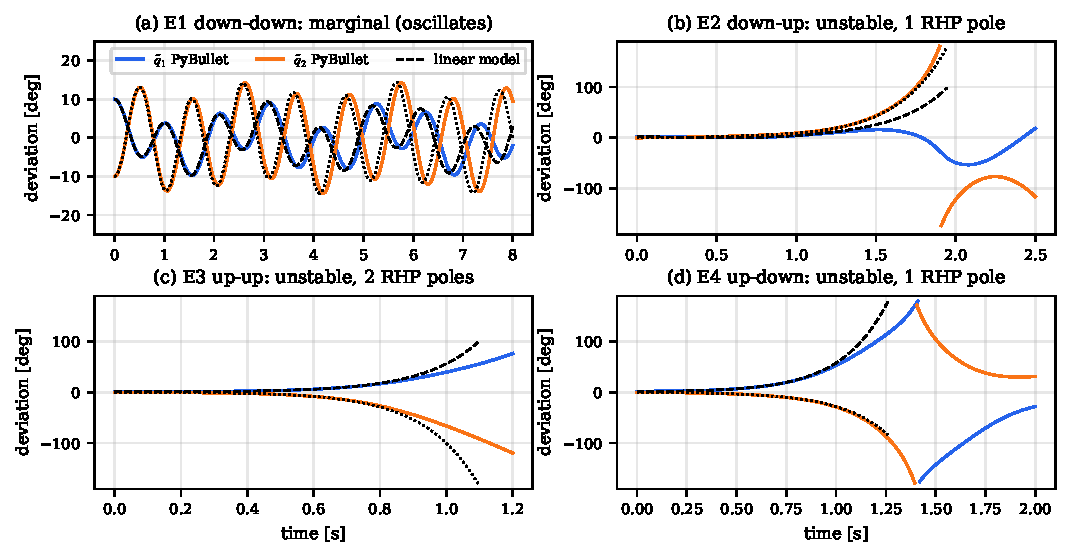
\includegraphics[width=\textwidth]{figures/fig_openloop.pdf}
\caption{Free response ($\tau=0$) near each equilibrium: PyBullet (colour) vs.\ linear model (black).}
\label{fig:ol}
\end{figure}
\begin{figure}[H]
\centering
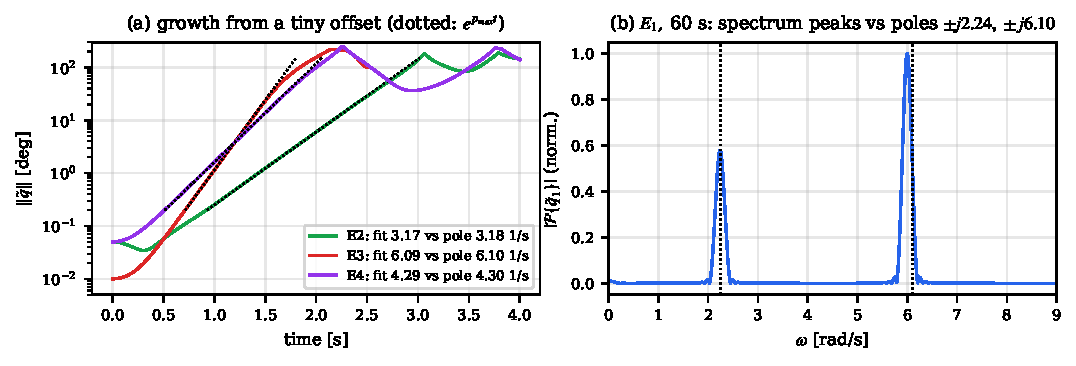
\includegraphics[width=\textwidth]{figures/fig_growth.pdf}
\caption{(a) Growth of a tiny offset on a log scale; dotted lines have the slope of the largest RHP pole. (b) Spectrum of $\tilde q_1$ near $E_1$; dotted lines are the poles.}
\label{fig:growth}
\end{figure}
\begin{table}[H]
\centering
\caption{Linear predictions vs.\ PyBullet measurements}
\label{tab:evidence}
\small
\begin{tabular}{|c|l|c|c|c|}
\hline
 & Quantity & Predicted & Measured & Error\\ \hline
$E_1$ & oscillation frequencies & $2.240,\ 6.101$ rad/s & $2.239,\ 5.997$ rad/s & within 1 bin\\
$E_1$ & energy change over 60 s & $0$ & $1.2\times10^{-3}$ J & integration error\\
$E_2$ & growth rate & $3.1775$ s$^{-1}$ & $3.171$ s$^{-1}$ & $0.22\%$\\
$E_3$ & growth rate & $6.1011$ s$^{-1}$ & $6.088$ s$^{-1}$ & $0.21\%$\\
$E_4$ & growth rate & $4.3010$ s$^{-1}$ & $4.294$ s$^{-1}$ & $0.15\%$\\ \hline
\end{tabular}
\end{table}
\textbf{Observations:}
\begin{itemize}
\item $E_1$ oscillates forever at its initial amplitude, with frequencies matching the poles.
\item A tiny offset at $E_2$, $E_3$, $E_4$ grows exponentially at exactly the rate of the largest RHP pole. At $E_3$ a $0.01^\circ$ tilt reaches $30^\circ$ in $1.55$~s.
\item The linear model tracks the nonlinear one until about $20^\circ$, then over-predicts.
\end{itemize}

\subsection{Can One Measured Angle Stabilize the Upright?}
\subsubsection{Static or PD Feedback}
Measuring one angle $y=\tilde q_j$ and applying $\tau=-(K_p+K_ds)\,y$ with $G_j=(b_2s^2+b_0)/(s^4+a_2s^2+a_0)$ gives the closed-loop polynomial
\begin{equation}
s^4+(K_db_2)\,s^3+(a_2+K_pb_2)\,s^2+(K_db_0)\,s+(a_0+K_pb_0) .\label{eq:pd}
\end{equation}
Hurwitz requires $K_db_2>0$ \emph{and} $K_db_0>0$, i.e.\ $b_2$ and $b_0$ of the same sign. At $E_3$:
\begin{itemize}
\item measuring $q_1$: $b_2=-3.0147$, $b_0=+12.6926$, opposite signs;
\item measuring $q_2$: $b_2=+6.0332$, $b_0=-31.7316$, opposite signs.
\end{itemize}
The signs are opposite because the zeros $\pm2.0519$ and $\pm2.2934$ are \textbf{real}: one of each pair lies in the right half-plane. \textbf{No $K_p$, $K_d$ can stabilize $E_3$ from one angle.} A grid search confirms it: the smallest attainable largest real part is $0.96$ ($q_1$) and $2.29$ ($q_2$), and in PyBullet even these gains fall from $1^\circ$ within 2~s.
\begin{figure}[H]
\centering
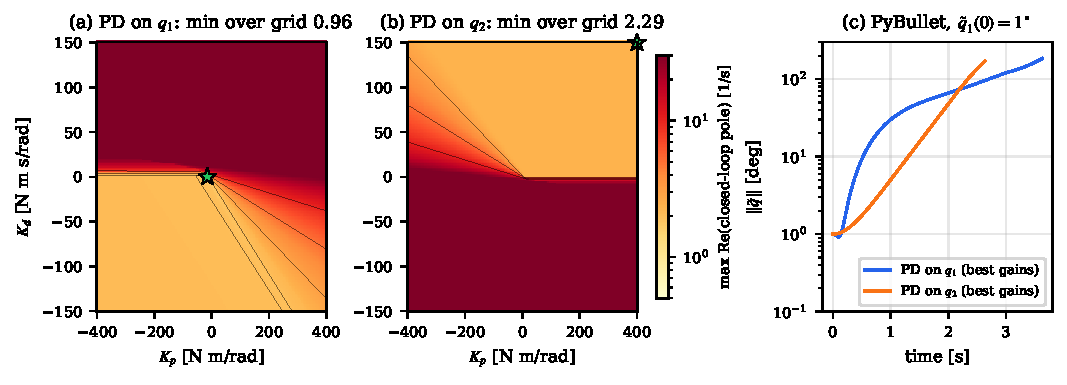
\includegraphics[width=\textwidth]{figures/fig_pd.pdf}
\caption{PD from one angle at $E_3$: (a, b) largest closed-loop real part over the gain plane, positive everywhere; (c) PyBullet with the best gains.}
\label{fig:pd}
\end{figure}

\subsubsection{Dynamic (Observer-Based) Feedback}
Each angle alone makes $(A,C_j)$ observable, so an observer can reconstruct the full state and LQR can act on the estimate:
\begin{equation}
\dot{\hat x}=A\hat x+B_\ell\tau+L(y-C_j\hat x),\qquad \tau=-K\hat x,\qquad \lambda_{cl}=\lambda(A-B_\ell K)\cup\lambda(A-LC_j).
\end{equation}
Two limits apply to \emph{any} controller:
\begin{itemize}
\item \textbf{Parity interlacing [6]:} for $q_1$ the interval $(2.05,\infty)$ contains two real RHP poles, so a stable controller suffices. For $q_2$, $(2.29,\infty)$ contains one, so the controller itself must be unstable.
\item \textbf{Sensitivity bound [3]:} $\|S\|_\infty\ge\prod_i|z+p_i|/|z-p_i|$, which is $\ge45.9$ for $q_1$ and $\ge187$ for $q_2$, because each zero sits just below the pole $2.24$.
\end{itemize}
In PyBullet the observer-based loop holds $E_3$ only from $1.42^\circ$ (measuring $q_1$) or $0.23^\circ$ (measuring $q_2$), against $4.64^\circ$ with full-state feedback.
\begin{figure}[H]
\centering
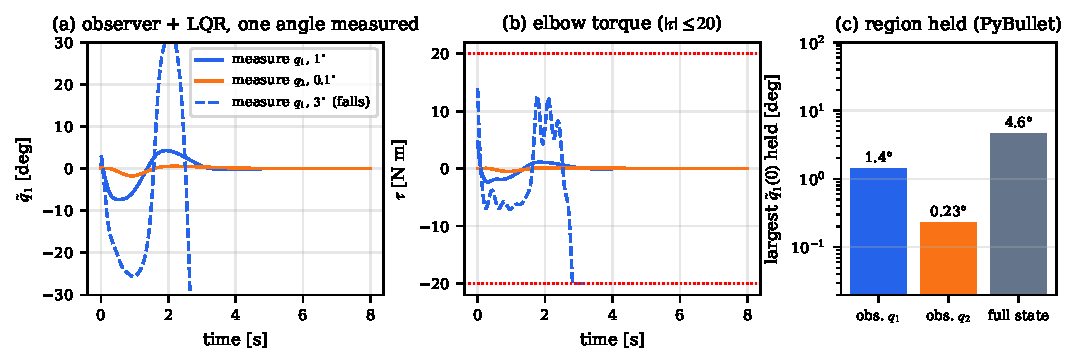
\includegraphics[width=\textwidth]{figures/fig_observer.pdf}
\caption{Observer + LQR at $E_3$ in PyBullet using one angle: (a) $\tilde q_1$; (b) torque; (c) largest initial offset held.}
\label{fig:obs}
\end{figure}
\textbf{Answer:} static or PD feedback from one joint angle \textbf{cannot} stabilize the upright, because of the real RHP zero. A dynamic controller \textbf{can}, but only for about a degree with $|\tau|\le20\Nm$, so Phase~3 uses full-state feedback.

% =====================================================================
% =====================================================================
\section{Simulations and Code}
% =====================================================================
\subsection{PyBullet Simulator}
All simulations use the full nonlinear model in PyBullet with an interactive dashboard (Fig.~\ref{fig:dash}). The user picks an equilibrium, an initial condition (slider, typed value or by dragging the arm) and a controller: open loop, PD on one angle (live $K_p$, $K_d$), or observer + LQR on one angle. The dashboard shows $\tilde q(t)$, $\tau(t)$ and the closed-loop poles live. File: \texttt{phase2/acrobot\_phase2\_sim.py}; instructions in \texttt{phase2/README.md}.
\begin{figure}[H]
\centering
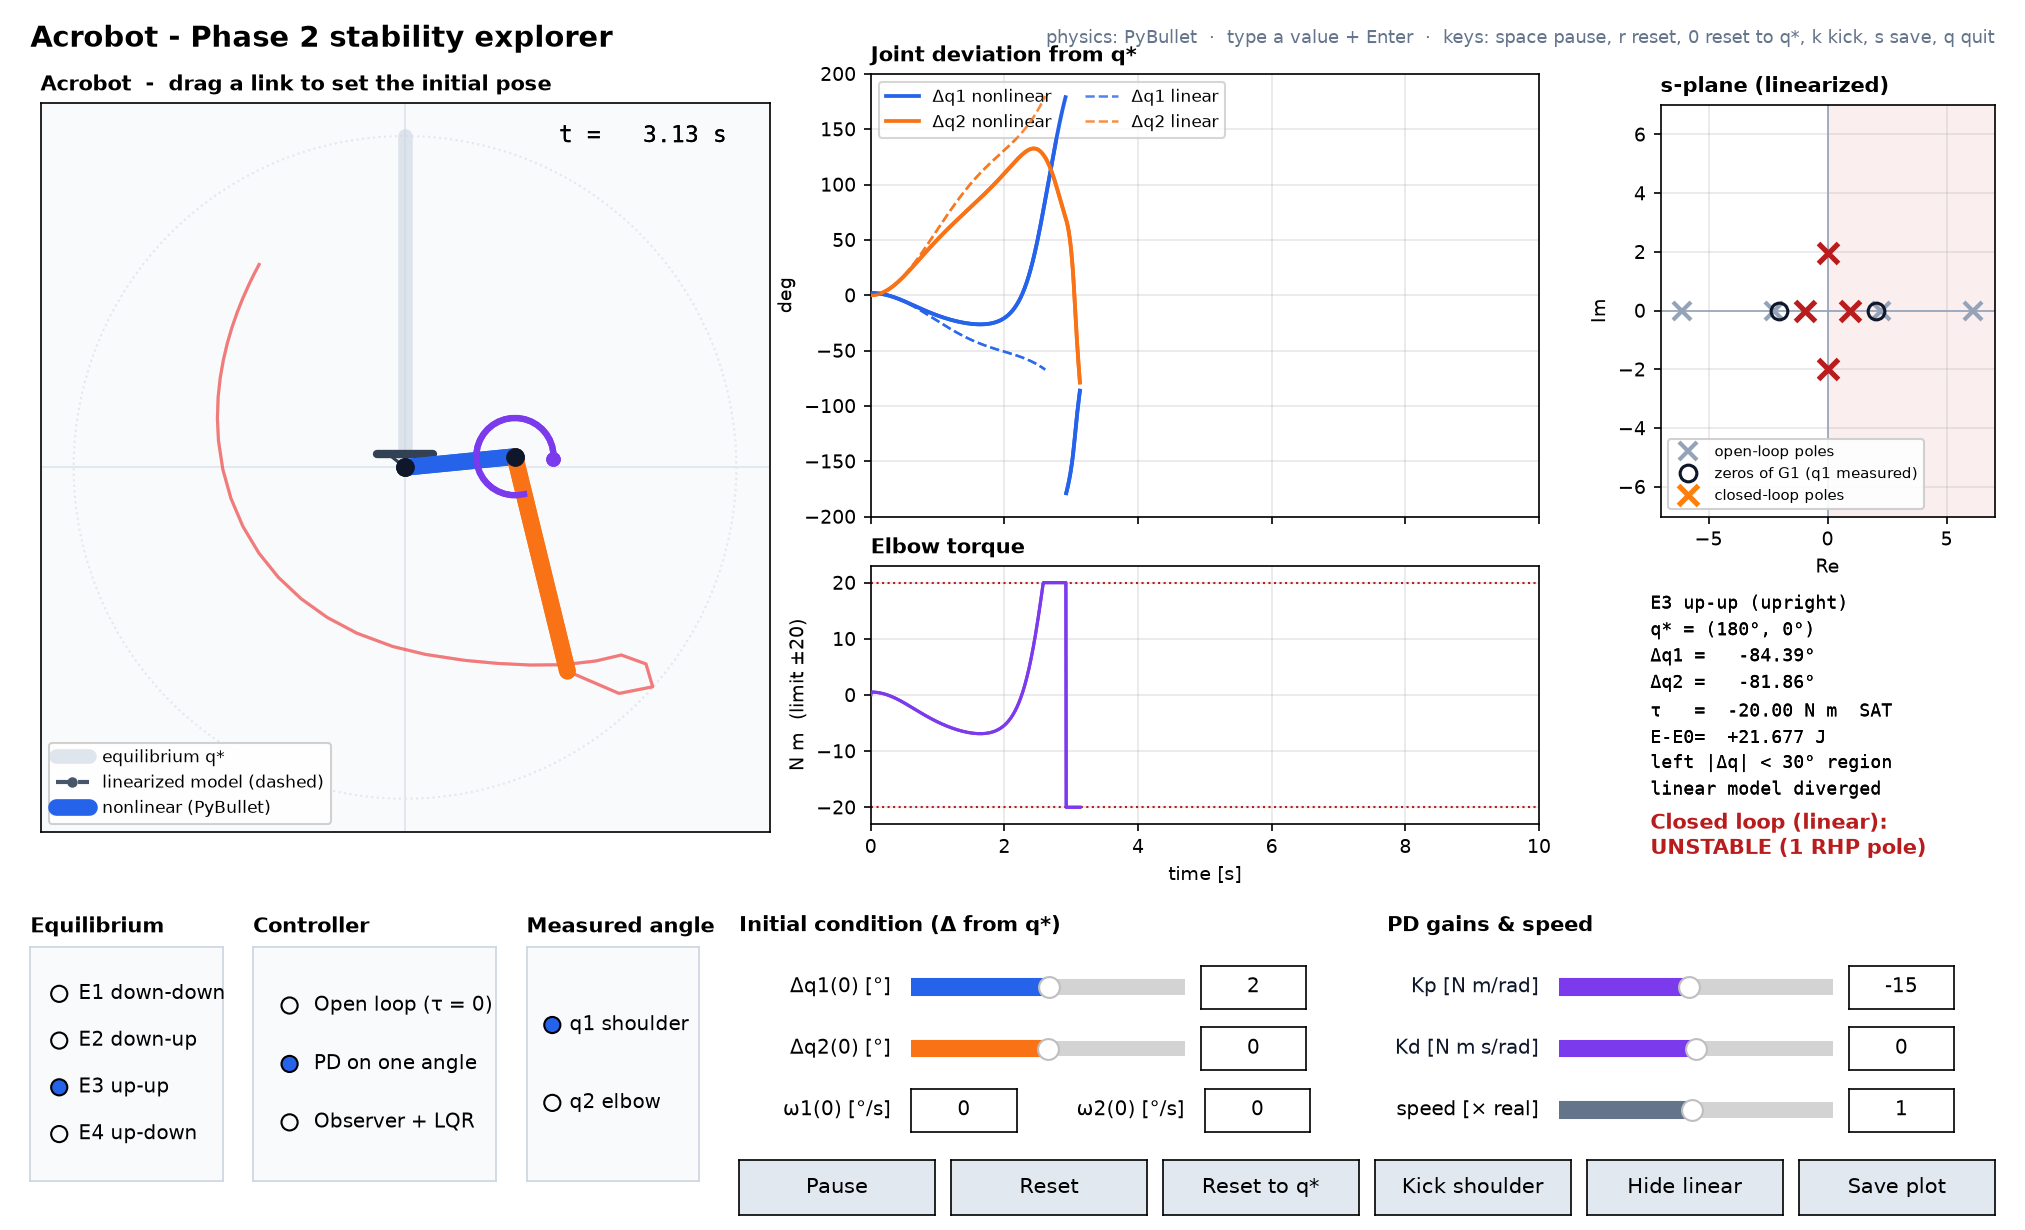
\includegraphics[width=\textwidth]{figures/dashboard_p2.png}
\caption{Phase 2 dashboard: PD on $q_1$ at the upright; a closed-loop pole stays in the right half-plane.}
\label{fig:dash}
\end{figure}

\subsection{MATLAB Codes}
It prints the poles, zeros, ranks and verdict for every equilibrium, measures the growth rates with \texttt{ode45}, and runs the single-angle PD search. Every number matches the tables above.

The files are listed below; the algorithms they implement follow as pseudo-code.
\begin{table}[H]
\centering
\caption{MATLAB files}
\resizebox{\textwidth}{!}{\begin{tabular}{|l|l|}
\hline
File & Purpose\\ \hline
\texttt{Acrobot\_Nonlinear\_Dynamics.m} & nonlinear model $\dot x=f(x,\tau)$ with the $20\Nm$ limit (Phase 1)\\
\texttt{Acrobot\_Linearize.m} & $A$, $B_\ell$ at an equilibrium (Phase 1)\\
\texttt{Acrobot\_Phase2\_Main.m} & poles, zeros, ranks, verdicts, growth rates, single-angle PD test\\ \hline
\end{tabular}}
\end{table}

\begin{algorithm}[H]
\caption{Nonlinear dynamics $\dot x=f(x,\tau)$ (\texttt{Acrobot\_Nonlinear\_Dynamics.m}) and linearization (\texttt{Acrobot\_Linearize.m})}
\label{alg:model}
\begin{algorithmic}[1]
\Function{Dynamics}{$x=[q_1,q_2,\dot q_1,\dot q_2]$, $\tau$}
  \State $\tau\gets\max(-20,\min(20,\tau))$ \Comment{motor limit}
  \State build $M(q)$, $C(q,\dot q)$ and $\tau_g(q)$ from the given model
  \State solve $M\,\ddot q=\tau_g+B\tau-C\dot q$ for $\ddot q$ \Comment{backslash, never $M^{-1}$}
  \State \Return $[\dot q;\ \ddot q]$
\EndFunction
\Function{Linearize}{$q^*$}
  \State $K\gets\partial\tau_g/\partial q$ at $q^*$; \quad $P\gets M(q^*)^{-1}K$; \quad $r\gets M(q^*)^{-1}B$
  \State \Return $A=\begin{bmatrix}0&I\\P&0\end{bmatrix}$, $B_\ell=\begin{bmatrix}0\\r\end{bmatrix}$
\EndFunction
\end{algorithmic}
\end{algorithm}

\begin{algorithm}[H]
\caption{Stability analysis and single-angle test (\texttt{Acrobot\_Phase2\_Main.m})}
\label{alg:p2}
\begin{algorithmic}[1]
\For{each equilibrium $E_k\in\{E_1,E_2,E_3,E_4\}$}
  \State $(A,B_\ell)\gets$ \Call{Linearize}{$q^*_k$}; \quad poles $\gets\operatorname{eig}(A)$
  \State $G_1,G_2\gets$ transfer functions $\tau\to q_1$, $\tau\to q_2$; \quad zeros $\gets$ roots of their numerators
  \State check $\operatorname{rank}\mathcal C=\operatorname{rank}\mathcal O_1=\operatorname{rank}\mathcal O_2=4$ \Comment{minimal: poles of $G_j$ = eig$(A)$}
  \State verdict $\gets$ asymptotically / marginally stable / unstable from the signs of $\operatorname{Re}(\text{poles})$
\EndFor
\For{$E_k\in\{E_2,E_3,E_4\}$} \Comment{nonlinear check}
  \State simulate $\tau=0$ from a $0.01^\circ$ offset (\texttt{ode45})
  \State fit the slope of $\ln\|\tilde q(t)\|$ and compare it with the largest RHP pole
\EndFor
\For{measured angle $j\in\{1,2\}$ at $E_3$} \Comment{PD from one angle}
  \State write $G_j=(b_2s^2+b_0)/\Delta(s)$
  \If{$b_2\,b_0<0$} \State PD is impossible (no Hurwitz $K_p,K_d$) \EndIf
  \State grid-search $(K_p,K_d)$: record the smallest $\max\operatorname{Re}\lambda(A-B_\ell F)$
\EndFor
\end{algorithmic}
\end{algorithm}


\subsection{Animation}
A 2K Manim animation of this phase: \href{https://drive.google.com/file/d/19THfoXXzbdMtbteCKE4v0VRLpV869wE0/view?usp=sharing}{\textcolor{blue}{watch the video}}.

% =====================================================================
\section{Tabulation}
% =====================================================================
\begin{table}[H]
\centering
\caption{Summary of the stability analysis}
\begin{tabular}{|c|c|c|c|}
\hline
Equilibrium & RHP poles & Energy shape & Stability\\ \hline
$E_1$ down--down & 0 & minimum & marginally (Lyapunov) stable\\
$E_2$ down--up & 1 & saddle & unstable\\
$E_3$ up--up & 2 & maximum & unstable\\
$E_4$ up--down & 1 & saddle & unstable\\ \hline
\end{tabular}
\end{table}
\begin{table}[H]
\centering
\caption{Single-angle feedback at the upright $E_3$ ($|\tau|\le20\Nm$)}
\resizebox{\textwidth}{!}{\begin{tabular}{|l|c|c|}
\hline
Controller & Measuring $q_1$ & Measuring $q_2$\\ \hline
PD (any $K_p$, $K_d$) & impossible (best $\max\operatorname{Re}\lambda=0.96$) & impossible (best $2.29$)\\
Observer + LQR & held up to $1.42^\circ$ & held up to $0.23^\circ$\\
Stable controller possible? & yes & no (must be unstable)\\
Sensitivity bound $\|S\|_\infty\ge$ & $45.9$ & $187$\\ \hline
\end{tabular}}
\end{table}

% =====================================================================
\section{Conclusion}
% =====================================================================
The acrobot has four zero-torque equilibria. Only the hanging pose $E_1$ is stable, and only in the Lyapunov sense: its poles lie on the imaginary axis and, with no friction, it oscillates forever. $E_2$ and $E_4$ have one RHP pole each (saddles of the potential energy) and the upright $E_3$ has two (a maximum), so all three are unstable. The transfer functions and the state matrix give the same verdicts because each realization is minimal, and PyBullet confirmed the predicted growth rates to within $0.25\%$.

A single measured angle cannot stabilize the upright with static or PD feedback: the real right-half-plane zeros of $G_1$ and $G_2$ make the required coefficient signs contradict each other. An observer-based dynamic controller can stabilize it, because each angle alone makes the system observable. With $|\tau|\le20\Nm$ it holds only about a degree, and via $q_2$ the controller would itself have to be unstable. This motivates full-state feedback in Phase~3.

% =====================================================================
\section{Contributions}
% =====================================================================
% Fill in who did what before submitting.
\begin{enumerate}
\item Report compilation -- \underline{\hspace{4cm}}
\item Stability criteria and analysis (Sections 2.1--2.5) -- \underline{\hspace{4cm}}
\item Simulation evidence (Section 2.6) -- \underline{\hspace{4cm}}
\item Single-angle feedback (Section 2.7) -- \underline{\hspace{4cm}}
\item PyBullet simulator and figures -- \underline{\hspace{4cm}}
\item MATLAB codes -- \underline{\hspace{4cm}}
\item Animation (Manim) -- \underline{\hspace{4cm}}
\end{enumerate}

\begin{thebibliography}{9}
\bibitem{spong} M.~W. Spong, ``The swing up control problem for the Acrobot,'' \emph{IEEE Control Systems Magazine}, vol.~15, no.~1, pp.~49--55, 1995.
\bibitem{tedrake} R.~Tedrake, \emph{Underactuated Robotics}, MIT, 2024. Available: https://underactuated.csail.mit.edu
\bibitem{skogestad} S.~Skogestad and I.~Postlethwaite, \emph{Multivariable Feedback Control}, 2nd ed., Wiley, 2005.
\bibitem{khalil} H.~K. Khalil, \emph{Nonlinear Systems}, 3rd ed., Prentice Hall, 2002.
\bibitem{pybullet} E.~Coumans and Y.~Bai, ``PyBullet, a Python module for physics simulation,'' 2016--2024. Available: https://pybullet.org
\bibitem{youla} D.~C. Youla, J.~J. Bongiorno and C.~N. Lu, ``Single-loop feedback-stabilization of linear multivariable dynamical plants,'' \emph{Automatica}, vol.~10, pp.~159--173, 1974.
\bibitem{anderson} B.~D.~O. Anderson and J.~B. Moore, \emph{Optimal Control: Linear Quadratic Methods}, Prentice Hall, 1990.
\end{thebibliography}

\end{document}
